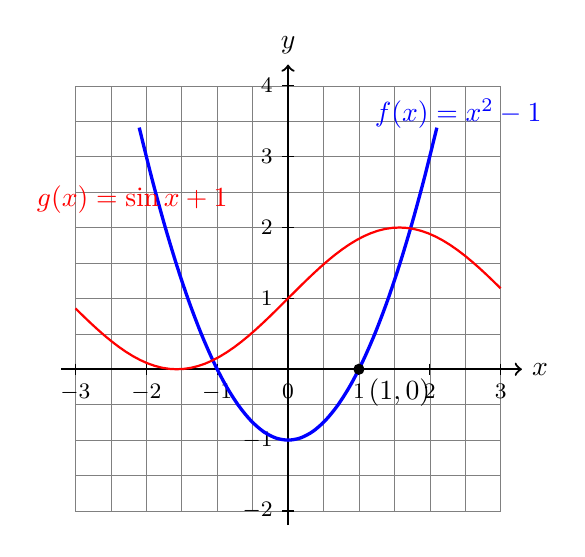
\begin{tikzpicture}[scale=0.9]
  \draw[help lines, step=0.5] (-3,-2) grid (3,4);
  \draw[->, thick] (-3.2,0) -- (3.3,0) node[right] {$x$};
  \draw[->, thick] (0,-2.2) -- (0,4.3) node[above] {$y$};
  \foreach \x in {-3,...,3} \draw (\x,0.08) -- (\x,-0.08) node[below] {\footnotesize $\x$};
  \foreach \y in {-2,-1,1,2,3,4} \draw (0.08,\y) -- (-0.08,\y) node[left] {\footnotesize $\y$};
  \draw[domain=-2.1:2.1, smooth, variable=\x, blue, very thick] plot ({\x}, {\x*\x - 1});
  \draw[domain=-3:3, samples=60, red, thick] plot (\x, {sin(\x r) + 1});
  \node[blue] at (2.4,3.6) {$f(x)=x^2-1$};
  \node[red] at (-2.2,2.4) {$g(x)=\sin x + 1$};
  \filldraw[black] (1,0) circle (2pt) node[below right] {$(1,0)$};
\end{tikzpicture}
